\documentclass[12pt]{report}
\usepackage{graphicx}
\usepackage[left=1.25in, top=1in, right=1in, bottom=1in]{geometry}
\usepackage{fontspec}
\setmainfont{Times New Roman}
\usepackage[base]{babel}
\usepackage{lipsum}
% \usepackage{amsmath}
% \usepackage{amssymb}
% \usepackage{tikz}
\usepackage[hidelinks]{hyperref}
\usepackage{tocloft}
\renewcommand{\contentsname}{\MakeUppercase{Table of Contents}}
\renewcommand{\cfttoctitlefont}{\hfill\Large\bfseries}
\renewcommand{\cftaftertoctitle}{\hfill\null{}}
\renewcommand{\listfigurename}{\MakeUppercase{List of Figures}}
\renewcommand{\cftloftitlefont}{\hfill\Large\bfseries}
\renewcommand{\cftafterloftitle}{\hfill}
\renewcommand{\listtablename}{\MakeUppercase{List of Tables}}
\renewcommand{\cftlottitlefont}{\hfill\Large\bfseries}
\renewcommand{\cftafterlottitle}{\hfill}
\usepackage[capitalize, nameinlink]{cleveref}
\usepackage{siunitx}
\usepackage{setspace}

\usepackage{tabularray}
\UseTblrLibrary{booktabs}

\usepackage{titlesec}
% \titleformat{command}[shape]{format}{label}{sep}{before-code}[after-code]
% \titlespacing*{command}{left}{before-sep}{after-sep}[right-sep]
%display %block %frame %hang %leftmargin %rightmargin %drop %wrap
\titleformat{\chapter}[display]{\bfseries\centering\fontsize{16}{0}\selectfont}{\MakeUppercase\chaptertitlename\ \thechapter}{10pt}{\MakeUppercase}
\titlespacing{\chapter}{0pt}{0pt}{10pt}

\titleformat{\section}[hang]{\bfseries\fontsize{14}{20}\selectfont}{\thesection}{15pt}{}
\titlespacing*{\section}{0pt}{0pt}{0pt}
%\titlespacing{\section}{Sp before (left) Section}{Sp above Section}{Sp below Section}

\titleformat{\subsection}[hang]{\bfseries\fontsize{12}{20}\selectfont}{\thesubsection}{15pt}{}
\titlespacing*{\subsection}{0pt}{0pt}{0pt}

% \usepackage{enumitem}
% \usepackage{minted}
\usepackage{luacode}
\directlua{dofile("data.lua")}

\usepackage{fancyhdr}
% \pagestyle{fancy}
% \fancyhf{}
% \cfoot{\thepage}
% \renewcommand{\headrulewidth}{0pt}

\usepackage[style=ieee]{biblatex}
\addbibresource{references.bib}
% \usepackage{showframe}

\renewcommand{\baselinestretch}{1.5}
\setlength{\parindent}{0.5in}
% \setlength{\parskip}{0pt}

\setcounter{secnumdepth}{3}

\begin{document}
\begin{titlepage}
    \centering
    
    
\includegraphics[width=3cm]{images/TribhuvanUniversityLogo.png}\par\vspace{1cm}
    
    {\par\noindent\large\bfseries\MakeUppercase{Tribhuvan University}}
    
    % \vspace{0.5cm}
    
    {\par\noindent\large\bfseries\MakeUppercase{Institute of Science and Technology}}
    
    \vspace{1.5cm}
    
    {\par\noindent\large\bfseries{A Project Proposal\par on}}
    
    {\par\noindent\Large\bfseries\MakeUppercase{A Short and Not So Long Project Title}}
    
    \vspace{3cm}
    
    {\par\large\bfseries Submitted By}
    {\par\large Apple (01234) \par Ball (6789A)}

    \vspace{1cm}

    {\par\large\bfseries Submitted To}
    {\par\large Cat}
    
    \vfill
    
    {\par\large\today}
\end{titlepage}

\pagenumbering{roman}
% certificates, acknowledgements, ...
\clearpage
\tableofcontents
\clearpage
\listoffigures
\clearpage
\listoftables

\clearpage
\setcounter{page}{1}
\pagenumbering{arabic}
\chapter{Introduction}

\section{Section One}

\lipsum[1-1] \cite{ValacichModernDesign}

\subsection{Section One One Two}
\lipsum[2-2]

\section{Section Two}

\lipsum[1-2] See \cref{fig:volcano}

\begin{figure}[htbp]
    \centering
    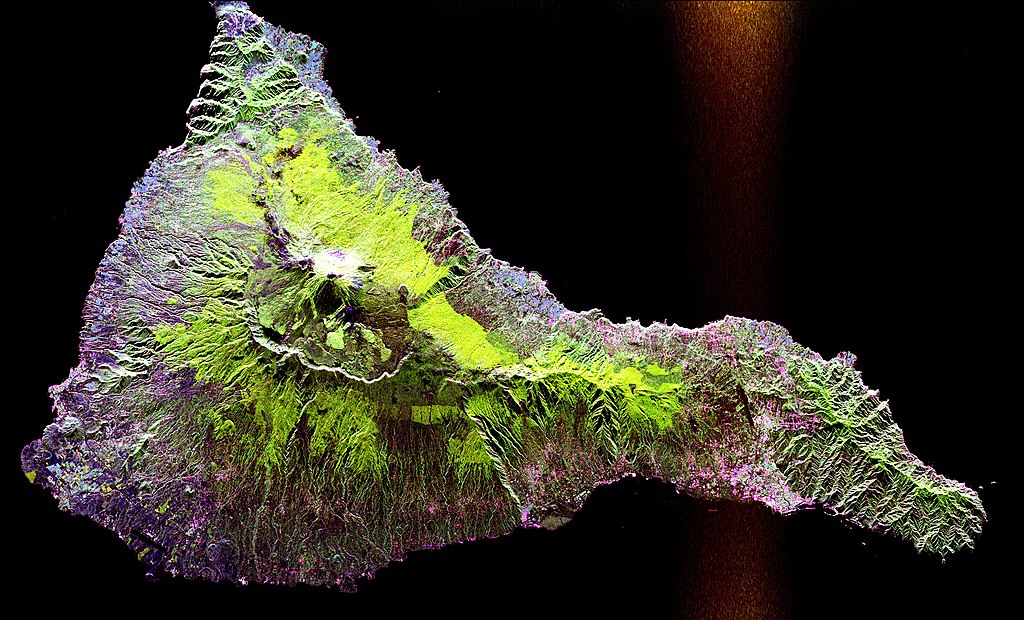
\includegraphics[width=0.5\linewidth]{images/volcano.JPG}
    \caption{Volcano}
    \label{fig:volcano}
\end{figure}
\chapter{Problem Statement}

\section{Section Two One}
\lipsum[1-2]

\begin{table}[htbp]
    \centering
    \begin{tblr}{llll}
    \toprule
    Alpha & Beta & Gamma & Delta \\
    \midrule
    Epsilon & Zeta & Eta & Theta \\
    \cmidrule{1-3}
    Iota & Kappa & Lambda & Mu \\
    \cmidrule{2-4}
    Nu & Xi & Omicron & Pi \\
    \bottomrule
    \end{tblr}
    \caption{Caption}
    \label{tab:my_label}
\end{table}

\printbibliography
\end{document}
